% This section is intended to be included via \input{} in a main paper file.
% Required packages in the main file: graphicx, tabularx.

\section{Experiments}
\label{sec:experiments}

\subsection{Dataset and Protocol}
\label{subsec:dataset-protocol}

Experiments are conducted on the Multi-Source Ship Trajectory Dataset (MSTD), which is collected from Bohai Bay in Shandong Province. The curated release used in this study contains 2,107 complete six-hour trajectory groups and 566,045 trajectory observations from three heterogeneous maritime monitoring systems: AIS, BDS, and shore-based radar. Each group provides associated trajectories from all three sources, but the trajectories are not point-wise aligned. The sources differ in sampling density, temporal continuity, spatial accuracy, and local noise distribution, making MSTD suitable for evaluating both multi-source completion and trajectory forecasting under realistic sensing heterogeneity.

Fig.~\ref{fig:mstd-visualization} visualizes the dataset from three complementary perspectives. The spatial coverage panel shows that the samples cover multiple traffic routes in the Bohai Bay region. The representative trajectory panels show that AIS, BDS, and Radar often describe similar vessel motion patterns while still exhibiting local offsets, different sampling densities, and source-specific noise. The statistical panels further quantify this heterogeneity: the median numbers of observations per sequence are 124 for BDS, 94 for AIS, and 54 for Radar, while the median sampling intervals are approximately 1.98 min for BDS, 1.98 min for AIS, and 4.98 min for Radar. These characteristics motivate a patch-level fusion model rather than direct point-wise replacement between sources.

\begin{figure*}[t]
    \centering
    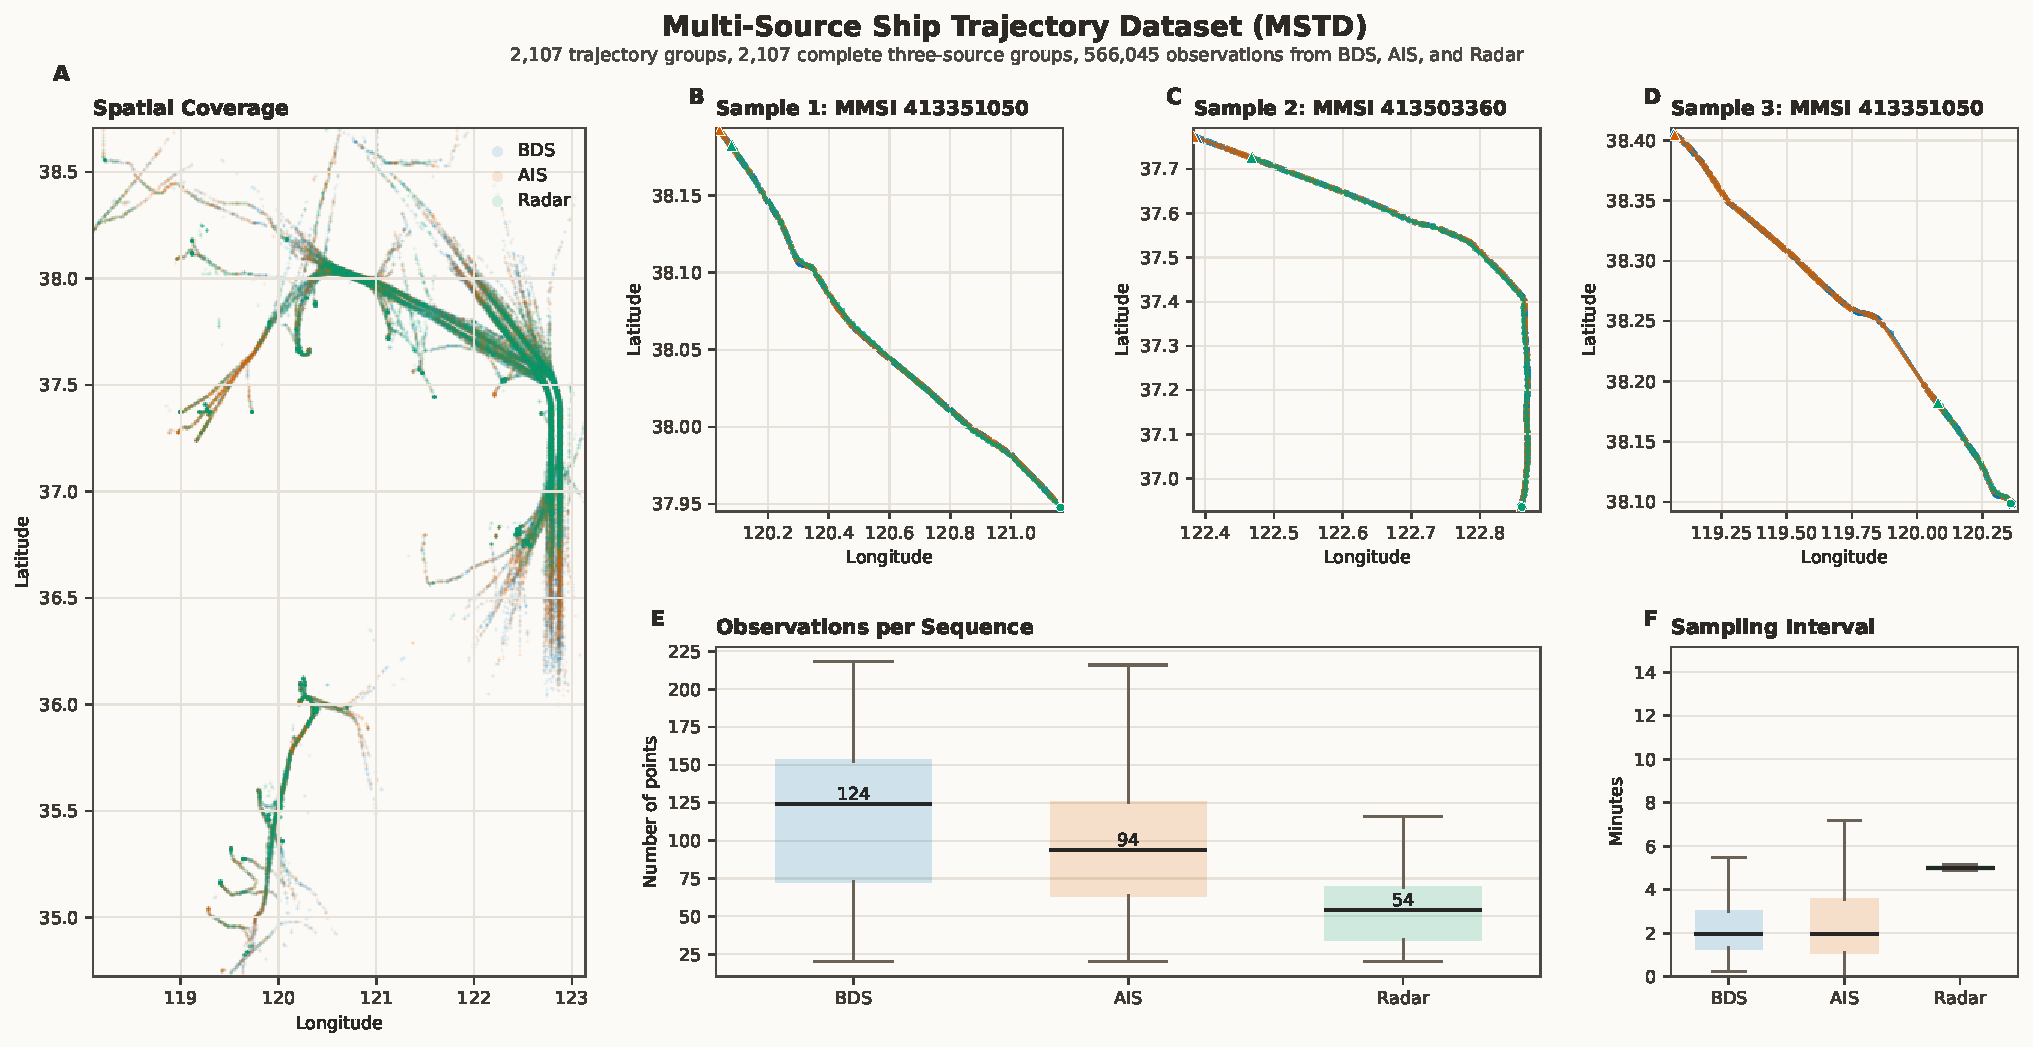
\includegraphics[width=0.99\textwidth]{figures/mstd_dataset_overview.pdf}
    \caption{Visualization of the Multi-Source Ship Trajectory Dataset (MSTD). Panel A shows the spatial coverage of BDS, AIS, and Radar observations. Panels B--D show representative associated three-source trajectory groups. Panels E and F summarize the distribution of observation counts and sampling intervals for each source. The figure highlights the weak alignment, unequal sampling density, and source-dependent continuity that motivate patch-level cross-source completion.}
    \label{fig:mstd-visualization}
\end{figure*}

For each sample, one source is selected as the target trajectory and the remaining sources are treated as optional auxiliary trajectories. This protocol supports three evaluation modes: single-source forecasting, single-auxiliary completion, and multi-auxiliary completion. Historical incompleteness is simulated using two corruption types. Empty-patch masking removes all observations inside selected historical patches, while sparse-patch masking keeps only a small number of observations in the selected patches to represent low-density monitoring regions.

All methods use the same train/validation/test split of 60\%/20\%/20\%, the same input history, the same prediction horizon, and the same normalization statistics. Hyperparameters are selected on the validation split, and the checkpoint with the lowest validation loss is evaluated on the test split. We report Test Loss, positional mean absolute error (Pos MAE), final-step mean absolute error (Final MAE), average L2 distance (Avg L2), average mean squared error (Avg MSE), and average dynamic time warping distance (Avg DTW). Lower values indicate better performance for all metrics.

\subsection{Overall Forecasting Performance}
\label{subsec:overall-performance}

The first experiment evaluates single-target forecasting without historical corruption. This setting isolates the ability of each model to encode irregular trajectory histories and predict future vessel motion before introducing auxiliary-source completion. The comparison includes classical recurrent models, patch-based time-series models, graph-based forecasting models, irregular time-series models, continuous-time models, and the proposed Traj-PathFormer. All baselines are trained and evaluated with the same no-sliding protocol so that each original trajectory group contributes only one training or testing sample.

Table~\ref{tab:overall-performance-mstd} reports the completed single-target forecasting results. Traj-PathFormer obtains the lowest Test Loss, Pos MAE, Final MAE, Avg L2, Avg MSE, and Avg DTW among the compared methods. The improvement over recurrent and continuous-time baselines indicates that time-aware patch encoding is useful for irregular maritime trajectories. The improvement over patch and graph forecasting baselines further suggests that trajectory-specific temporal queries and local patch modeling are important for ship motion extrapolation.

\begin{table*}[t]
    \centering
    \caption{Single-target no-sliding forecasting performance. Lower is better for all metrics.}
    \label{tab:overall-performance-mstd}
    \small
    \begin{tabular}{lcccccc}
        \hline
        Method & Test Loss & Pos MAE & Final MAE & Avg L2 & Avg MSE & Avg DTW \\
        \hline
        Ours & 0.0912 & 221.3403 & 396.6012 & 0.003260 & 0.00001875 & 0.032463 \\
        AGDN & 0.1672 & 322.9428 & 568.9746 & 0.004701 & 0.00003416 & 0.045685 \\
        TLSTM & 0.1533 & 304.1389 & 534.5453 & 0.004457 & 0.00003063 & 0.043179 \\
        T-PatchGNN & 0.3515 & 632.3910 & 1148.7339 & 0.009282 & 0.00008465 & 0.107036 \\
        DLinear & 0.1468 & 296.5776 & 520.4579 & 0.004362 & 0.00002915 & 0.043687 \\
        TimesNet & 0.1608 & 320.3552 & 549.0652 & 0.004652 & 0.00002963 & 0.045639 \\
        PatchTST & 0.1607 & 342.7858 & 597.5205 & 0.005077 & 0.00003174 & 0.051094 \\
        Crossformer & 0.1327 & 294.1077 & 503.8624 & 0.004281 & 0.00002766 & 0.041038 \\
        Graph WaveNet & 0.1621 & 316.8399 & 539.9712 & 0.004603 & 0.00003175 & 0.045384 \\
        MTGNN & 0.1725 & 320.6826 & 553.6057 & 0.004723 & 0.00003397 & 0.046464 \\
        StemGNN & 0.1513 & 301.2865 & 534.9033 & 0.004445 & 0.00002788 & 0.045406 \\
        CrossGNN & 0.1470 & 291.3072 & 509.4098 & 0.004220 & 0.00002559 & 0.041731 \\
        FourierGNN & 0.1424 & 304.4529 & 527.9481 & 0.004438 & 0.00002473 & 0.044792 \\
        GRU-D & 0.1505 & 299.0100 & 516.3393 & 0.004419 & 0.00002861 & 0.042718 \\
        SeFT & 0.3007 & 532.1498 & 987.2258 & 0.007802 & 0.00007024 & 0.086307 \\
        RainDrop & 0.2072 & 393.5482 & 732.4191 & 0.005834 & 0.00004123 & 0.058391 \\
        Warpformer & 0.1456 & 293.2483 & 519.3995 & 0.004280 & 0.00002633 & 0.042219 \\
        mTAND & 0.3154 & 572.5056 & 1027.1610 & 0.008375 & 0.00007512 & 0.092223 \\
        Latent-ODE & 0.1449 & 291.9276 & 505.7471 & 0.004294 & 0.00002745 & 0.041619 \\
        CRU & 0.1520 & 306.5746 & 537.9244 & 0.004482 & 0.00003031 & 0.043251 \\
        Neural Flow & 0.1305 & 274.2642 & 480.2103 & 0.004070 & 0.00002432 & 0.040065 \\
        \hline
    \end{tabular}
\end{table*}

\subsection{Robustness to Incomplete Historical Patches}
\label{subsec:missing-sparse-robustness}

The second experiment evaluates whether patch-level completion improves forecasting when historical observations are incomplete. We consider two types of incomplete history. Empty-patch corruption represents complete local sensing failure, where all observations in selected patches are removed. Sparse-patch corruption represents low-density monitoring, where only a few observations remain inside the selected patches. For each corruption level, we compare three protocols: forecasting without completion, direct source filling, and the proposed single-source cross-attention completion.

Table~\ref{tab:missing-sparse-robustness} shows that cross-attention completion consistently gives the best results across both empty and sparse patch settings. Direct source filling can reduce error when a target patch is fully empty, but it is less reliable under sparse corruption because copying auxiliary points may overwrite useful target observations or introduce source-specific offsets. In contrast, cross-attention completion transfers information at the representation level, allowing the model to use auxiliary evidence while preserving the target trajectory context.

\begin{table*}[t]
    \centering
    \caption{Robustness to empty and sparse historical patches. Lower is better for all metrics.}
    \label{tab:missing-sparse-robustness}
    \small
    \begin{tabularx}{\textwidth}{llXcccccc}
        \hline
        Corruption & Patches & Completion Protocol & Test Loss & Pos MAE & Final MAE & Avg L2 & Avg MSE & Avg DTW \\
        \hline
        Empty & 1 & None & 0.0426 & 214.0463 & 349.9421 & 0.003177 & 0.00001376 & 0.032712 \\
        Empty & 1 & Direct Source Fill & 0.0418 & 204.6442 & 332.9675 & 0.003037 & 0.00001315 & 0.031304 \\
        Empty & 1 & Single-Source Cross-Attn. & 0.0410 & 202.6891 & 330.3001 & 0.003009 & 0.00001291 & 0.031109 \\
        \hline
        Empty & 2 & None & 0.0434 & 219.3537 & 360.6593 & 0.003259 & 0.00001433 & 0.033507 \\
        Empty & 2 & Direct Source Fill & 0.0431 & 208.9927 & 340.5367 & 0.003099 & 0.00001380 & 0.031884 \\
        Empty & 2 & Single-Source Cross-Attn. & 0.0412 & 203.3165 & 331.3052 & 0.003016 & 0.00001305 & 0.031164 \\
        \hline
        Empty & 3 & None & 0.0439 & 220.9296 & 364.7376 & 0.003283 & 0.00001458 & 0.033825 \\
        Empty & 3 & Direct Source Fill & 0.0433 & 209.8891 & 341.9404 & 0.003113 & 0.00001376 & 0.032073 \\
        Empty & 3 & Single-Source Cross-Attn. & 0.0413 & 203.0973 & 331.0697 & 0.003012 & 0.00001298 & 0.031154 \\
        \hline
        Sparse & 1 & None & 0.0413 & 205.1377 & 334.2994 & 0.003044 & 0.00001301 & 0.031408 \\
        Sparse & 1 & Direct Source Fill & 0.0418 & 204.6442 & 332.9675 & 0.003037 & 0.00001315 & 0.031304 \\
        Sparse & 1 & Single-Source Cross-Attn. & 0.0409 & 202.3945 & 329.7261 & 0.003005 & 0.00001287 & 0.031072 \\
        \hline
        Sparse & 2 & None & 0.0416 & 206.4329 & 336.1953 & 0.003064 & 0.00001309 & 0.031566 \\
        Sparse & 2 & Direct Source Fill & 0.0431 & 208.9927 & 340.5367 & 0.003099 & 0.00001380 & 0.031884 \\
        Sparse & 2 & Single-Source Cross-Attn. & 0.0410 & 202.7830 & 330.3737 & 0.003010 & 0.00001297 & 0.031107 \\
        \hline
        Sparse & 3 & None & 0.0419 & 207.1303 & 337.2458 & 0.003072 & 0.00001312 & 0.031643 \\
        Sparse & 3 & Direct Source Fill & 0.0433 & 209.8891 & 341.9404 & 0.003113 & 0.00001376 & 0.032073 \\
        Sparse & 3 & Single-Source Cross-Attn. & 0.0410 & 202.5264 & 330.1328 & 0.003005 & 0.00001290 & 0.031089 \\
        \hline
    \end{tabularx}
\end{table*}

\subsection{Single-Source and Multi-Source Completion}
\label{subsec:source-completion-analysis}

The third experiment studies which auxiliary source should be used for completion. One source is selected as the target trajectory, while the other sources are used individually or jointly. The single-source setting uses one auxiliary local patch sequence. The multi-source setting uses two auxiliary local patch sequences, each with length three, and fuses them through cross-attention before reconstructing the incomplete target patch. This design evaluates whether Radar, AIS, and BDS provide complementary evidence rather than interchangeable point-wise replacements.

Table~\ref{tab:source-completion-analysis} defines the source-selection comparison for one incomplete target patch. The rows are organized by target source so that the effect of each auxiliary source can be interpreted separately. The ``None'' rows measure the cost of making predictions from incomplete target history alone. The single-source rows measure how much each auxiliary source contributes individually. The multi-source rows test whether jointly attending to two auxiliary sources provides a stronger and more stable completion signal.

\begin{table*}[t]
    \centering
    \caption{Effect of auxiliary source selection for one incomplete target patch. Lower is better for all metrics.}
    \label{tab:source-completion-analysis}
    \small
    \begin{tabularx}{\textwidth}{llXcccccc}
        \hline
        Target & Auxiliary Source(s) & Completion Protocol & Test Loss & Pos MAE & Final MAE & Avg L2 & Avg MSE & Avg DTW \\
        \hline
        AIS & None & No Completion & -- & -- & -- & -- & -- & -- \\
        AIS & BDS & Single-Source Cross-Attn. & -- & -- & -- & -- & -- & -- \\
        AIS & Radar & Single-Source Cross-Attn. & -- & -- & -- & -- & -- & -- \\
        AIS & BDS + Radar & Multi-Source Cross-Attn. & -- & -- & -- & -- & -- & -- \\
        \hline
        BDS & None & No Completion & -- & -- & -- & -- & -- & -- \\
        BDS & AIS & Single-Source Cross-Attn. & -- & -- & -- & -- & -- & -- \\
        BDS & Radar & Single-Source Cross-Attn. & -- & -- & -- & -- & -- & -- \\
        BDS & AIS + Radar & Multi-Source Cross-Attn. & -- & -- & -- & -- & -- & -- \\
        \hline
        Radar & None & No Completion & -- & -- & -- & -- & -- & -- \\
        Radar & AIS & Single-Source Cross-Attn. & -- & -- & -- & -- & -- & -- \\
        Radar & BDS & Single-Source Cross-Attn. & -- & -- & -- & -- & -- & -- \\
        Radar & AIS + BDS & Multi-Source Cross-Attn. & -- & -- & -- & -- & -- & -- \\
        \hline
    \end{tabularx}
\end{table*}

\subsection{Local Auxiliary Patch Length}
\label{subsec:local-patch-length-ablation}

The fourth experiment verifies the choice of using three auxiliary patches for local cross-attention completion. A very short auxiliary context may not contain enough motion evidence when the target patch is missing or sparse. Conversely, a long auxiliary context may introduce temporally distant observations that are weakly related to the missing target region. We therefore compare interpolation, direct source filling, and cross-attention completion with one to eight auxiliary patches.

Table~\ref{tab:local-patch-length-ablation} is structured to identify the best local auxiliary window. The interpolation and direct-filling rows are non-attention baselines, while the cross-attention rows test how the model behaves as the auxiliary context grows. The expected operating point is the smallest window that provides stable gains without adding distant-source noise or unnecessary computation.

\begin{table*}[t]
    \centering
    \caption{Ablation on the number of auxiliary patches used for completion. Lower is better for all metrics.}
    \label{tab:local-patch-length-ablation}
    \small
    \begin{tabularx}{\textwidth}{lXcccccc}
        \hline
        Strategy & Auxiliary Context & Test Loss & Pos MAE & Final MAE & Avg L2 & Avg MSE & Avg DTW \\
        \hline
        Linear Interpolation & Target source only & -- & -- & -- & -- & -- & -- \\
        Direct Source Fill & One auxiliary source & -- & -- & -- & -- & -- & -- \\
        Cross-Attn. & 1 auxiliary patch & -- & -- & -- & -- & -- & -- \\
        Cross-Attn. & 2 auxiliary patches & -- & -- & -- & -- & -- & -- \\
        Cross-Attn. & 3 auxiliary patches & -- & -- & -- & -- & -- & -- \\
        Cross-Attn. & 4 auxiliary patches & -- & -- & -- & -- & -- & -- \\
        Cross-Attn. & 5 auxiliary patches & -- & -- & -- & -- & -- & -- \\
        Cross-Attn. & 6 auxiliary patches & -- & -- & -- & -- & -- & -- \\
        Cross-Attn. & 7 auxiliary patches & -- & -- & -- & -- & -- & -- \\
        Cross-Attn. & 8 auxiliary patches & -- & -- & -- & -- & -- & -- \\
        \hline
    \end{tabularx}
\end{table*}

\subsection{Model Ablation}
\label{subsec:ablation-study}

The final experiment evaluates the contribution of the main architectural components. Each variant removes or replaces one design while keeping the dataset split, corruption protocol, training schedule, and evaluation metrics fixed. This controlled setting separates the effect of time-aware encoding, future-step querying, completion, multi-source fusion, temporal patch bias, and intra-patch modeling.

Table~\ref{tab:model-ablation} lists the planned ablation variants. The full model corresponds to Traj-PathFormer with time-aware patch embedding, temporal patch attention, local cross-attention completion, and the time-conditioned future query decoder. The ablated variants are chosen to answer whether each component is necessary, whether direct source filling can replace learned completion, and whether multi-source fusion provides benefits beyond a single auxiliary trajectory.

\begin{table*}[t]
    \centering
    \caption{Model ablation on MSTD. Lower is better for all metrics.}
    \label{tab:model-ablation}
    \small
    \begin{tabularx}{\textwidth}{lXcccccc}
        \hline
        Variant & Description & Test Loss & Pos MAE & Final MAE & Avg L2 & Avg MSE & Avg DTW \\
        \hline
        Full Model & Complete Traj-PathFormer & -- & -- & -- & -- & -- & -- \\
        w/o Time-Aware Encoding & Remove temporal interval encoding from patch and future queries & -- & -- & -- & -- & -- & -- \\
        w/o Future Query Decoder & Replace time-conditioned future queries with a global prediction head & -- & -- & -- & -- & -- & -- \\
        w/o Completion Branch & Predict from incomplete history without patch completion & -- & -- & -- & -- & -- & -- \\
        Direct Source Fill & Replace cross-attention completion with direct auxiliary-source filling & -- & -- & -- & -- & -- & -- \\
        Single-Source Completion Only & Disable multi-source auxiliary fusion & -- & -- & -- & -- & -- & -- \\
        w/o Temporal Patch Bias & Replace temporally biased patch attention with standard self-attention & -- & -- & -- & -- & -- & -- \\
        w/o Intra-Patch Attention & Replace point-level intra-patch attention with masked mean pooling & -- & -- & -- & -- & -- & -- \\
        \hline
    \end{tabularx}
\end{table*}
